{
{\sffamily Vi vil i dette kapitel se på, hvilke resultater, vi med vores
metoder, er kommet frem til. Vi præsenterer en række hypoteser og
undersøger hvorvidt vores data kan be- eller afkræfte disse hypoteser.
Vi vil også gerne se, om vores data fremvise nogle interessante
observationer vedrørende kunstneres oprindelse eller fødselsår.
}

\section{Hypoteser}
{
{\sffamily Vi vil i det følgende præsentere de hypoteser, som vi, på
baggrund af resultaterne af den efterfølgende analyse på vores datasæt,
vil forsøge at verificere. De fleste af hypoteserne antager den
generelle opfattelse, at det gyldne snit er specielt æstetisk tiltalende
og af denne grund, er meget brugt i malerkunsten. Sidst i afsnittet vil
vi kaste et kritisk blik på vores datasæt, for at se på hvad vi kan
forvente af vores analyse.
}

\begin{hypotese}
    Hvis det gyldne snit er meget brugt i malerkunsten, må vi have, at
    over halvdelen, af de analyserede malerier, har én eller flere
    regioner liggende i det gyldne snit.
\end{hypotese}

\emph{eller}

\begin{hypotese}
    I en analyse på et stort antal malerier, vil over halvdelen af disse
    have mindst én region i det gyldne snit, da det gyldne snit bliver
    brugt meget i malerkunsten.
\end{hypotese}

\emph{eller}

\begin{hypotese}
    Det gyldne snit er meget brugt i malerkunsten, da over halvdelen, af
    de analyserede malerier, har én eller flere regioner liggende i det
    gyldne snit.
    \label{hypo_binaer}
\end{hypotese}

\hrule

\begin{hypotese}
    Hvis et gyldent snit er specielt æstetisk tiltalende, må vi have, at
    antallet af regioner liggende hvert af de fire snit, som kan
    betragtes som gyldne, ikke afviger mere end $\pm10\%$ fra hinanden.
\end{hypotese}

\emph{eller}

\begin{hypotese}
    Et gyldent snit er specielt æstetisk tiltalende, da antallet af
    regioner, liggende i hvert af de fire gyldne snit, ikke afviger med
    mere end $\pm10\%$ fra hinanden.
\end{hypotese}

\hrule

\begin{hypotese}
    Hvis det gyldne rektangel er et specielt æstetisk tiltalende format,
    må vi have, at mere end en tredjedel malerierne har et lærred, hvis
    dimensioner er lig $\varphi\pm2.4\%$.
\end{hypotese}

\emph{eller}

\begin{hypotese}
    Det gyldne rektangel er et specielt æstetisk tiltalende format,
    fordi mere end en tredjedel af alle malerier, har et lærred, hvor
    forholdet mellem dimensionerne  er lig $\varphi\pm2.4\%$.
\end{hypotese}

\hrule

\begin{hypotese}
    Hvis det gyldne snit er bevidst brugt af kunstneren, må vi have, at
    antallet regioner liggende i det gyldne snit, er skarpt større, end
    antallet af regioner liggende i snittet ved to tredjedele.
    \label{hypo_golden_ractangle}
\end{hypotese}

\emph{eller}

\begin{hypotese}
    Det gyldne snit bruges bevidst af kunstnere, da der findes flere
    regioner i det gyldne snit, end i snittet ved to tredjedele.
	\label{hypototredjedele}
\end{hypotese}

\hrule

\begin{hypotese}
    Hvis det gyldne snit er meget brug i malerkunsten, må vi have, at
    antallet af detekterede regioner i det gyldne snit, er skarpt
    større, end antallet i alle andre snit.
\end{hypotese}

\emph{eller}

\begin{hypotese}
    Det gyldne snit er meget brugt i malerkunsten, fordi der findes
    flere regioner i det gyldne snit end antallet af regioner liggende i
    ethvert andet snit.
	\label{hypoethvertandetsnit}
\end{hypotese}

\hrule

\begin{hypotese}
    Hvis det gyldne snit er bevidst brugt af kunstneren, må vi have, at
    antallet regioner liggende i det gyldne snit, er skarpt større, end
    antallet af regioner liggende det midterste snit.
\end{hypotese}

\emph{eller}

\begin{hypotese}
    Det gyldne snit bruges bevidst af kunstnere, da der findes flere
    regioner liggende i det gyldne snit end antallet af regioner
    liggende i det midterste snit.
	\label{hypomidten}
\end{hypotese}

\hrule

\begin{hypotese}
    Hvis det gyldne snit altid har været specielt æstetisk tiltalende,
    må vi have, at antallet af regioner liggende i det gyldne snit,
    tidsperioder imellem, højest kan afvige med $\pm10\%$.
\end{hypotese}

\emph{eller}

\begin{hypotese}
    Det gyldne snit har altid været lige meget brugt i malerkunsten, fordi
    antallet af regioner i det gyldne snit, tidsperioder imellem, kun
    afviger med $\pm10\%$.
\end{hypotese}

\hrule

\begin{hypotese}
    Hvis det gyldne snit er ligeså  æstetisk tiltalende for alle,
    må vi have, at antallet af regioner liggende i det gyldne snit,
    nationaliteter imellem, højest kan afvige med $\pm10\%$.
\end{hypotese}

\emph{eller}

\begin{hypotese}
    Det gyldne snit er lige æstetisk tiltalende for alle, fordi antallet
    af regioner liggende i det gyldne snit, nationaliteter imellem, kun
    afviger med $\pm10\%$.
\end{hypotese}

\hrule

\begin{hypotese}
    Hvis det gyldne snit er specielt æstetisk tiltalende, og vi har at
    \emph{the rule of thirds} bliver brugt i malerkunsten, som en
    approksimation til det gyldne snit, må vi have, at antallet af
    regioner liggende i det gyldne snit ikke angiver fra antallet af
    regioner i to tredjedele med mere end $15\%$.
\end{hypotese}

\emph{eller}

\begin{hypotese}
    \emph{The Rule of Thirds} bliver brugt i malerkunsten som en
    approksimation til det gyldne snit, fordi antallet af regioner, som
    findes i det gyldne snit, ikke afviger med mere end $\pm15\%$ fra
    antallet af regioner, som findes i snittet ved to tredjedele.
\end{hypotese}

\subsection{Datasæt}
Det korpus, vi kører vores analyse på, består af billeder hentet fra
``The Web Gallery of Art''\cite{wgahu}, som er en online billededatabase, med
europæiske kunstartikler fra år 1001 -- 1900. I kunstartiklerne, hvor
det samlede antal er omkring 23.000, indgår møbler, kalkmalerier,
skulpturer, mosaikker og malerier, hvor sidstnævnte, vil være vores
fokus. Over halvdelen af disse kunstartikler står udstillet på museum.
Databasen blev oprettet i 1996, med det formål at præsentere kunst fra
renæssancen (ca.  14. -- 17.  århundrede), men blev senere udvidet, til
også at inkludere kunst fra andre perioder. Dette betyder, at
størstedelen af malerierne vi undersøger, er fra tidsperioden 1450 --
1650 og er malet af italienske kunstnere. Endvidere er langt de fleste
malerier, klassificeret som religiøse.  Disse informationer er givet fra
WGA, men er også suppleret i bilag \ref{appendix_grafer} som
grafer.

Vi må af ovenstående grunde forvente, at resultater, fra en analyse på
vores datasæt, vil være farvet af samlingen af malerier, og det derfor
kan være svært at drage nogen konklusioner for malerkunsten generelt, da
resultaterne vil være begrænset, til kun at gælde for et udsnit af
vestlig kultur. Endvidere findes der ingen nyere malerier i datasættet,
hvilket gør at vi ikke kan udtale os om nyere malerkunst.

Billederne, som suppleres fra databasen, er af høj kvalitet, men der er
visse problemer, som vi nævner nedenfor.

\begin{itemize}
    \item \textbf{Beskæring af billeder}\\
        Vi kan ikke vide os sikre på, om billederne i datasættet er
        ordentligt beskåret, hvilket betyder at vi \emph{kan} have, at
        noget af billedrammen er med i billedet. Dette kan muligvis
        volde lidt problemer med udtrækning af regioner, men hvad værre
        er, så gør det vores mål, for hvor det gyldne snit ligger,
        upræcist. Dette har vi dog taget højde for, i kraft af vores
        margin.  Endeligt er der inkluderet billeder af malerier
        detaljer i databasen, som er udsnit af maleriet, således at
        målene på billedet ikke passer.
    \item \textbf{Forvrængning og perspektiv}\\
        Billederne af malerier er taget med et kamera, hvor linsen muligvis kan
        forvrænge billedet. Vi kan derfor have skæve linjer og tage
        forkerte beslutninger, for regioner, pga. dette. Endvidere kan
        billedet være taget skævt, således at billedet hælder til den
        ene side. Vi kan selvfølgelig også have at perspektivet i
        billedet er forkert, fordi billedet er taget fra en skæv vinkel.
    \item \textbf{Opdelte malerier}\\
        Nogle store malerier kan være blevet opdelt, da databasen har
        det formål at vise malerierne på en computerskærm, hvor meget
        store billeder kan være svære at betragte. Dette betyder, at
        nogle billeder ikke viser hele maleriet, men blot er et udsnit,
        hvilket påvirker vores muligheder for at sige noget fornuftigt
        om det gyldne snit i maleriet.
\end{itemize}

Nogle stilarter, såsom kalkmalerier og tegninger, har gennem
udokumenterede afprøvninger, vist sig at være besværlige at analysere,
pga. meget svingende farvegengivelse. Endvidere, kan disse være billeder
af en hvælving i en kirke, som ikke egner sig til analyse for det gyldne
snit. Vi har derfor valgt kun at analysere malerier, kendetegnet ved at
de er beskrevet som ``painting'' fra WGA.

Alt det ovenstående vil påvirke resultaterne, ved analyse på vores
datasæt.

}
% vim: set tw=72 spell spelllang=da:


\section{Kørsel af naiv implementering\label{section_naiv_koersel}}
{
{\sffamily I det følgende vil vi samle op på resultaterne fra det kørte
eksperiment med den naive vurdering af regioner. Vores metode til
udtrækning af regioner, har dog indeholdt en fejl, som vi først vil
beskrive.
}

\subsection{Systematisk fejl\label{program_bug}}
I den naive løsning findes en fejl i udtrækningen af regioner, som gør
at vi finder nogle af
regionerne flere gange. Denne fejl nævnt i afsnit
\ref{section_impBilledbehandling} og gennemgået i bilag
\ref{appendix_bug}. Det betyder, at de resultater vi fremviser for kørslen
af den naive løsning, ikke helt passer. For at give en indblik i, hvor
mange regioner der bliver fundet flere gange, har vi afprøvet programmet med
fejlen på 11 malerier, og sammenlignet dem med en kørsel, hvor fejlen er
rettet.

De 11 malerier er opstillet i tabel \ref{bug_tabel}, hvor de to første
kolonner er antal regioner fundet i billedet, uden og med fejl.  Tredje
kolonne er en procentsats for, hvor mange flere regioner der bliver
fundet, når den fejlende kode køres. Den procentvise spredning er $[60
\%,~377 \%]$, så de resultater vi får, kan være op til $377\%$ for høje.
Gennemsnitligt er der $172 \%$ flere regioner. Vi kan godt antage, at
antallet af regioner opgivet i resultaterne for den naive løsning, er
halv så store.

\begin{table}[!h]
    \centering
    \begin{tabular}{|l|c|c|c|}
        \hline
  Maleri  & Bug løst 		& Bug ikke løst		& Procentvis forskel\\\hline
        1   & 70 			& 112 				& 60 \% \\
        2   & 27 			& 45 				& 67 \% \\
        3	& 52 			& 98 				& 72 \% \\
        4   & 84 			& 145 				& 73 \% \\
        5	& 32 			& 57 				& 78 \% \\
        6   & 88 			& 170 				& 93 \% \\
        7   & 85 			& 201 				& 136 \% \\
        8   & 78 			& 197 				& 153 \% \\
        9   & 164 			& 554 				& 238 \% \\
        10	& 16 			& 75 				& 368 \% \\
        11	& 115 			& 548 				& 377 \% \\\hline
	Total	& 881			& 2202				& 172 \% \\\hline
	  \end{tabular}
    \caption[]{Tabel for antal fundne regioner i versionen med og uden
    fejlen som duplikerer regioner. Den sidste kolonne er hvor mange
    procent flere regioner der bliver fundet.}
    \label{bug_tabel}
\end{table}

\clearpage

\subsection{Resultater}
Vi har kørt analyse med naiv vurdering på $17,364$ malerier, men i vores
resultater sorterer vi $2,989$ af disse fra, da de kun er udsnit af et
større maleri.  Som vist i tabel \ref{tabel_fjern_detaljer} herunder, er
dette en nedgang på $17.21$ procent og vi har $14,375$ brugbare
resultater tilbage.

\begin{table}[H]
    \centering
    \begin{tabular}{r@{\ \ }p{12em}r|r@{.}l}
            & Analyserede malerier & $17,364$ & $100$ & $00\%$   \\
        $-$ & Udsnit af malerier   &  $2,989$ &  $17$ & $21\%$   \\\hline
            & Resultater           & $14,375$ &  $82$ & $79\%$
    \end{tabular}
    \caption[]{Udregning af brugbare resultater.}
    \label{tabel_fjern_detaljer}
\end{table}

Af de brugbare resultater, ser vi i tabel \ref{tabel_fordeling}, at der
i $91.43$ procent af malerierne er fundet mindst én region som ligger i
det gyldne snit. Vi kan derfor ikke afvise hypotese \ref{hypo_binaer}.

\begin{table}[H]
    \centering
    \begin{tabular}{r@{\ \ }p{12em}r|r@{.}l}
            & Positive resultater   & $13,143$ &  $91$ & $43\%$ \\
        $+$ & Negative resultater   &  $1,232$ &   $8$ & $57\%$ \\\hline
            & Resultater i alt      & $14,375$ & $100$ & $00\%$
    \end{tabular}
    \caption[]{Et positivt resultat beskriver et maleri, hvori der er
    fundet mindst én region, som ligger i det gyldne snit. Et negativt
    resultat er et maleri, hvori der ikke findes nogen regioner, som
    ligger i det gyldne snit.}
    \label{tabel_fordeling}
\end{table}

Vi vil gerne se på, hvordan fordelingen af fundne interessante regioner i
de fire gyldne snit ser ud. Fordelingen er vist i tabel
\ref{tabel_fire_snit}. Vi ser, at ingen af snittene afviger med mere end
$\pm10\%$ fra et andet og vi kan derfor ikke afvise hypotese
\ref{hypo_fire_g_snit}.

\begin{table}[H]
    \centering
    \begin{tabular}{r@{\ \ }p{12em}r|r@{.}l}
            & Regioner i snit 0   &  $42,884$ &  $24$ & $51\%$ \\
        $+$ & Regioner i snit 1   &  $44,042$ &  $25$ & $18\%$ \\
        $+$ & Regioner i snit 2   &  $46,432$ &  $26$ & $54\%$ \\
        $+$ & Regioner i snit 3   &  $41,547$ &  $23$ & $75\%$ \\\hline
            & Regioner i alt      & $168,650$ & $100$ & $00\%$
    \end{tabular}
    \caption[]{Forholdet mellem de interessante regioner fundet i de
    fire gyldne snit. Intet snit afviger med mere end $10\%$ fundne
    regioner, end et andet snit.}
    \label{tabel_fire_snit}
\end{table}

Vi undersøger nu, hvor mange af de brugbare resultater, som er forsynet
med dimensioner i databasen, således at vi kan undersøge, hvorvidt
lærredet er konstrueret som et gyldent rektangel. Udregningen i tabel
\ref{tabel_med_dimensioner} viser at ud af de brugbare resultater,
mangler $2,410$ malerier dimensionerne, og vi har da $11,965$ malerier
tilbage at undersøge, for den gyldne ratio i lærredets dimensioner.

\begin{table}[H]
    \centering
    \begin{tabular}{r@{\ \ }p{14em}r|r@{.}l}
            & Resultater                     & $14,375$ & $100$ & $00\%$ \\
        $-$ & Resultater uden dimensioner    &  $2,410$ &  $16$ & $77\%$ \\\hline
            & Resultater med dimensioner     & $11,965$ &  $83$ & $23\%$
    \end{tabular}
    \caption[]{Brugbare resultater med dimensioner i databasen.}
    \label{tabel_med_dimensioner}
\end{table}

Vi ser nu, hvor mange af de $11,965$ malerier, der har, at dets lange
side, $L$, divideret med dets korte side, $K$, ligger i intervallet $G =
[1.57920117302, 1.65686680448] = \varphi \pm 2.4\%$. Tabel
\ref{tabel_real_dimensions} viser, at kun $3.99\%$ falder inden for
dette interval. Vi kan således afvise hypotese
\ref{hypo_golden_ractangle}.

\begin{table}[H]
    \centering
    \begin{tabular}{r@{\ \ }p{14em}r|r@{.}l}
            & $L/K \in G$                  &    $478$ &   $3$ & $99\%$ \\
        $+$ & $L/K \notin G$               & $11,487$ &  $96$ & $01\%$ \\\hline
            & Resultater med dimensioner   & $11,965$ & $100$ & $00\%$
    \end{tabular}
    \caption[]{Resultater med dimensioner, hvor disse er et gyldent
    rektangel med en afvigelse på $2.4\%$. Under en tredjedel af
    malerierne har et lærred med gyldne dimensioner.}
    \label{tabel_real_dimensions}
\end{table}

\begin{table}[H]
    \centering
    \begin{tabular}{|c|l|c|c|}
		\hline
        \textbf{Hypotese nr.} & \textbf{Beskrivelse} & \textbf{Afvist} &
        \textbf{Ikke afvist}  \\\hline\hline
        1 & Mindst én region i $GS$                     &            & \checkmark   \\\hline
        2 & Alle fire $GS$ lige meget brugt             &            & \checkmark   \\\hline
        3 & $1/3$ har lærred med forholdet $1:\varphi $ & \checkmark &              \\\hline
        4 & Flest regioner i $GS$                       & \checkmark &              \\\hline
        5 & Flere regioner i $GS$ end $\frac{2}{3}$     &            & \checkmark   \\\hline
        6 & Flere regioner i $GS$ end i midten          & \checkmark &              \\\hline
        7 & $GS$ brugt lige meget, uanset tidsperiode   & \checkmark &              \\\hline
        8 & $GS$ brugt lige meget, uanset nationalitet  & \checkmark &              \\\hline
        9 & $\frac{2}{3}$ brugt som approksimation til $GS$   &            & \checkmark	\\\hline
    \end{tabular}
    \caption[]{Hypoteser i forhold til den naive kørsel. $GS$ bruges som
    forkortelse for det gyldne snit.}
    \label{hypoteser_naiv}
\end{table}

\subsubsection{Antallet af fundne regioner over alle snit}
I alle $14,375$ malerier er der i alt fundet $1,650,082$ interessante
regioner. Vi har en middelværdi på $114.79$ med standardafvigelse på
$86.91$. I figur \ref{total_regions_plots} er vist grafer over hvordan
antallet af fundne regioner fordeler sig i malerierne. I figur
\ref{graf_total_regions_zoom}, hvor der ses bort fra $298$ malerier,
hvori der ikke er fundet nogen regioner. Regionerne i malerierne har en
fordeling, der kunne ligne en eksponentialfordeling, som vist i
histogrammet i figur \ref{hist_total_regions}. De observerede værdier
fraviger dog noget fra de teoretiske værdier.

\begin{figure}[!h]
    \centering
    \subfloat[]{
        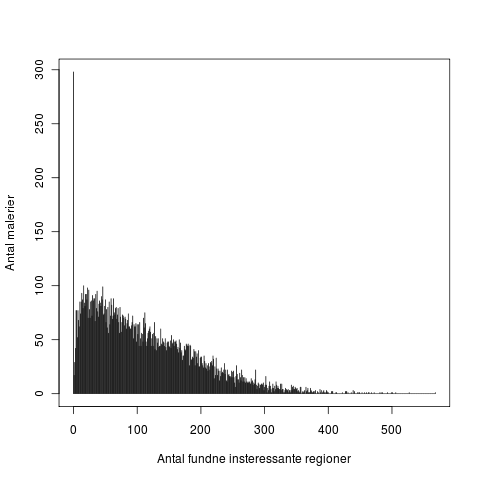
\includegraphics[width=0.49\textwidth]{afsnit/resultater/billeder/totalregions_var}
        \label{graf_total_regions_var}
    }
    \subfloat[]{
        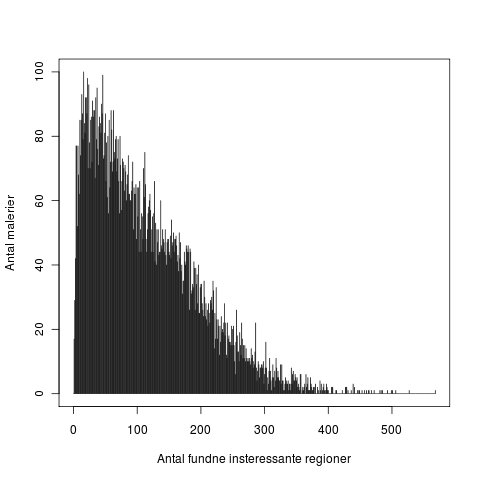
\includegraphics[width=0.49\textwidth]{afsnit/resultater/billeder/totalregions}
        \label{graf_total_regions_zoom}
    }\\
    \subfloat[]{
        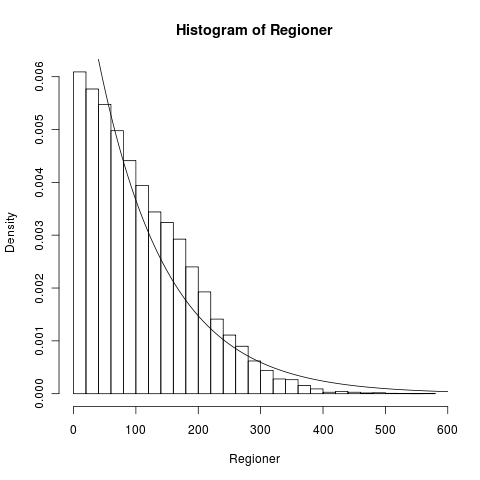
\includegraphics[width=0.62\textwidth]{afsnit/resultater/billeder/hist_totalregions}
        \label{hist_total_regions}
    }
    \caption[]{Fordelingen af fundne regioner på malerier.
    \textbf{\ref{graf_total_regions_var}:} Plot som viser hvor mange
    malerier, hvori der er fundet et vist antal interessante regioner
    over alle snit i maleriet.  \textbf{\ref{graf_total_regions_zoom}:}
    Samme plot som i figur \ref{graf_total_regions_var}, men hvor antal
    malerier uden regioner ikke er vist.
    \textbf{\ref{hist_total_regions}:} Histogram over antal fundne
    regioner, hvor en eksponentialfordeling med $\lambda = 1/109.82$ er
    indtegnet.}
    \label{total_regions_plots}
\end{figure}

Vi ser, at et maleri typisk har omkring $110$ interessante regioner i
alle snit. Her skal man være opmærksom på, at hver region meget vel
indgår fire gange. Vi ser, at der er et lille antal malerier, hvori der
bliver fundet rigtig mange regioner. Det tynder dog ud omkring
$380$ regioner, hvor antallet af malerier, med flere regioner,
forekommer mindre hyppigt.

Vi skal være opmærksomme på, at der kan være duplikater af regionerne.

}

% vim: set tw=72 spell spelllang=da:

\clearpage

Det må man sige at han er, og derfor er der ikke nogle grund til at lave
rastte af resultaterne da han bare kan ændre på virkeligheden.

Vi har køre vores naive algoritme på 20 snit i det horisontale og
vertikale plan og kommer frem til to grafer over summeringen af alle
regioner fundet i vært snit. 

Man kan se i grafen \ref{antal_regioner_vertikale_cut} for det vertikale
plan, at regionerne koncentrationen sig omkring miden af billederne.

I grafen for den horisontale plan \ref{antal_regioner_horisontale_cut}
er der tre snit som udskiller sig fra resten $91\%$, $61\%$ og $56\%$.
Hvor $91\%$ ligger højest. Fra miden af billedet og op af bliver der
fundet færre og færre regioner i snittene. Det kan skyldes at billeder med
hoisont normalt ikke har mange regioner over hoisonden, men mange under
hoisonden, eller at vores algoritme regner forkert, det første er nok det meste
sansyndlige, da vores algoritme iterere hoisontal i gemme maleriet nå vi skal
finde hoisontal regioner og vertikal nå vi finder vertikal regioner, så er
eventuel type fejl i algoritmen vil også kunne ses i den anden graf
\ref{antal_regioner_vertikale_cut}.

Hvis man samler informatioerne for de to grafer, kan man se at regionerne
samler sig fra den horisontale miden og ned af i billedet med peaker i
miden af det vertikalle plan. Det mod skrider hypotese \ref{hypo_alle_andre_snit} og \ref{hypo_midten}
og vi kan derfor forkaste dem.

I graferne kan vi også se at det gyldne snit $G$ har samme antal eller
flere regioner en $\frac{2}{3}$, som approksimmeret i grafen er $31$ og
$66$, derfor er hypotese \ref{hypo_to_tredjedele} sand og kan derfor ikke forkastes.

\begin{figure}[h!]
	\begin{center}
		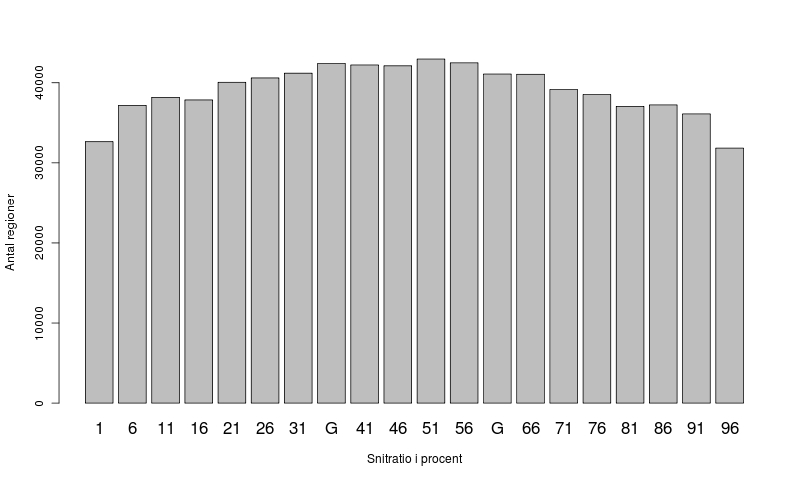
\includegraphics[width=0.9\textwidth]{afsnit/resultater/billeder/cut0cut1eatsperratio.png}
	\end{center}
	\caption{Antal regioner i hvert af de 20 vertikale snit}
	\label{antal_regioner_vertikale_cut}
\end{figure}

\begin{figure}[h!]
	\begin{center}
		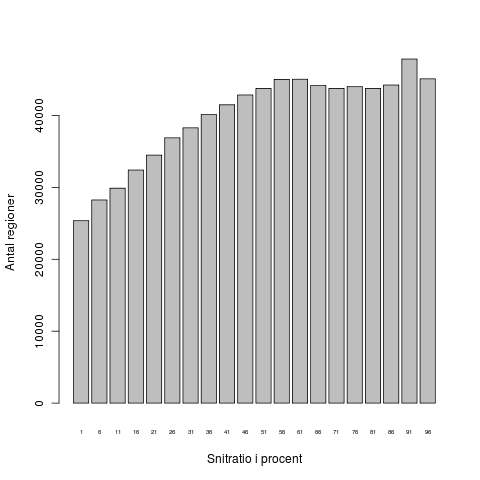
\includegraphics[width=0.9\textwidth]{afsnit/resultater/billeder/cut2cut3eatsperratio.png}
	\end{center}
	\caption{Antal regioner i hvert af de 20 horisontale snit, hvor venstre side af grafen repræsentere øverst del af malerierne}
	\label{antal_regioner_horisontale_cut}
\end{figure}

\clearpage

\section{Udvidet implementation\label{section_udvidet_koersel}}
{
{\sffamily Dette afsnit vil præsentere vores resultater fra
eksperimentet, hvor vi har brugt den udvidede metode, til at vurdere
regionerne. Da eksperimentet blev kørt, har vi sat opløsningen på
regionernes approksimation med et gitter for højt, hvilket har
resulteret i, at vi kun har 524 brugbare resultater til rådighed. Dette
svare til $\mathsf{3.65\%}$ af de brugbare resultater fra den naive
kørsel. Vores datasæt bliver gennemgået alfabetisk efter kunstnerens
efternavn, så vi har kun resultater fra kunstnere med efternavn
startende med 'A' og 'B'.
}

\subsection{Håndtering af systematisk fejl}
Selvom denne analyse også har brugt den fejlbehæftede metode, til
udtrækning af regioner, så sorteres duplikater fra, når vi approksimerer
en region. Vi har gemt farven, som en region er blevet tildelt af
floodfill, og hvis denne farve ikke er at finde i regionens begrænsende
rektangel, betyder det, at regionen er blevet malet over senere. Vi
smider derfor denne region væk.

Den udvidede metode indeholder derfor ingen duplikater, men resultaterne
er ikke direkte sammenlignelige med dem fra den naive kørsel.

\subsection{Resultater}
Vi har i denne kørsel analyseret $608$ malerier, men som vist herunder i
udregning \ref{ud_tabel_fjern_detaljer}, har vi kun $524$ brugbare
resultater, når vi har fjernet de billeder, som ikke er hele malerier.
Dette svarer til en nedgang på $13.82\%$.

\begin{table}[H]
    \centering
    \begin{tabular}{r@{\ \ }p{12em}r|r@{.}l}
            & Analyserede malerier & $608$ & $100$ & $00\%$   \\
        $-$ & Udsnit af malerier   &  $84$ &  $13$ & $82\%$   \\\hline
            & Resultater           & $524$ &  $86$ & $18\%$
    \end{tabular}
    \caption[]{Udregning af brugbare resultater fra udvidet kørsel.}
    \label{ud_tabel_fjern_detaljer}
\end{table}

I udregning \ref{ud_tabel_fordeling} herunder undersøger vi, hvor mange
af de brugbare resultater, som har mindst en region liggende i det
gyldne snit. Vi har at der i $87.02\%$ af malerierne er blevet fundet
regioner i det gyldne snit, og vi kan derfor ikke afvise hypotese
\ref{hypo_binaer}.

\begin{table}[H]
    \centering
    \begin{tabular}{r@{\ \ }p{12em}r|r@{.}l}
            & Positive resultater   & $456$ &  $87$ & $02\%$ \\
        $+$ & Negative resultater   &  $68$ &  $12$ & $98\%$ \\\hline
            & Resultater i alt      & $524$ & $100$ & $00\%$
    \end{tabular}
    \caption[]{Et positivt resultat beskriver et maleri hvori der er
    fundet mindst en region i det gyldne snit, ved brug af den udvidede
    vurdering af regioner.}
    \label{ud_tabel_fordeling}
\end{table}

Fordelingen af regioner, over de fire gyldne snit i malerierne, ses i
udregning \ref{ud_tabel_fire_snit}. Intet af de fire snit afviger med
mere end $10\%$ fra et andet, og vi kan således ikke afvise hypotese
\ref{hypo_fire_g_snit}.

\begin{table}[H]
    \centering
    \begin{tabular}{r@{\ \ }p{12em}r|r@{.}l}
            & Regioner i snit 0   &  $405$ &  $22$ & $29\%$ \\
        $+$ & Regioner i snit 1   &  $421$ &  $23$ & $17\%$ \\
        $+$ & Regioner i snit 2   &  $499$ &  $27$ & $46\%$ \\
        $+$ & Regioner i snit 3   &  $492$ &  $27$ & $08\%$ \\\hline
            & Regioner i alt      & $1817$ & $100$ & $00\%$
    \end{tabular}
    \caption[]{Forholdet mellem de interessante regioner fundet i de
    fire gyldne snit ved udvidet vurdering.}
    \label{ud_tabel_fire_snit}
\end{table}

% Spacer! Ikke over denne linje HAHAHA

I graf \ref{antal_regioner_vertikale_cut_udvidet} er der afbilledet,
antale sammelet regioner i de 20 vertikale snit for helle datasættet.
Som man kan se er der fundet makant flere regioner i de to snit som
ligger tættest på miden, og færest ud i kanterne. 

\begin{figure}[h!]
	\begin{center}
		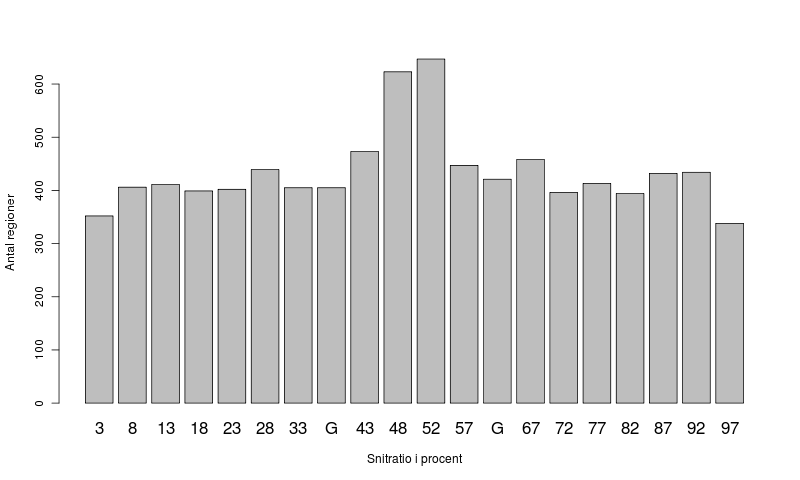
\includegraphics[width=0.9\textwidth]{afsnit/resultater/billeder/cut0cut1eatsperratioU.png}
	\end{center}
	\caption{Antal regioner i hvert af de 20 vertikale snit}
	\label{antal_regioner_vertikale_cut_udvidet}
\end{figure}

I graf \ref{antal_regioner_horisontale_cut_udvidet} er der samme
afbildning lavet, bare i det hoisontale plan, med venster side af grafen
svare til toppen af billedet. I denne graf er det 72,82 som peaker. Fra
52 og ned af, falder antal regioner gradvis. hvor i mod fra 52 og op gå
grafen lidt op og lidt ned. Kanterne er igen klart de lavest i grafen.

\begin{figure}[h!]
	\begin{center}
		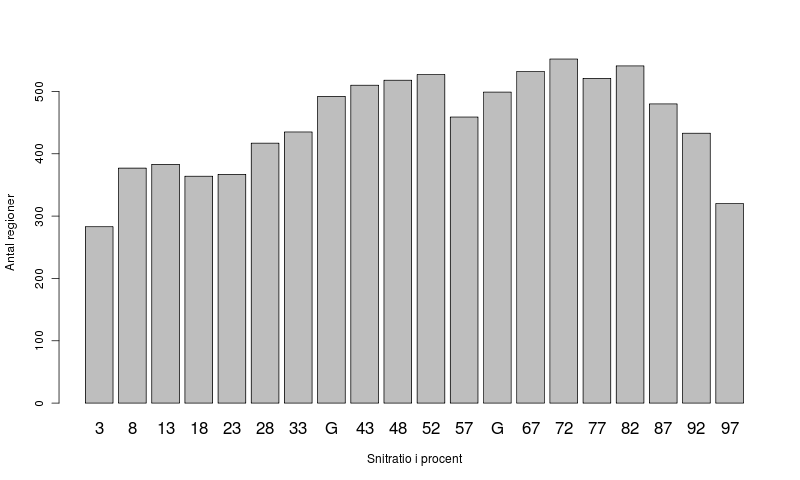
\includegraphics[width=0.9\textwidth]{afsnit/resultater/billeder/cut2cut3eatsperratioU.png}
	\end{center}
	\caption{Antal regioner i hvert af de 20 horisontale snit, hvor venstre side af grafen repræsentere øverst del af malerierne}
	\label{antal_regioner_horisontale_cut_udvidet}
\end{figure}

Ud fra disse observationer kan vi konkludere at der ikke er flere
regioner i det gyldne snit, en midden af billedet, og kan derfor
forkaste hypotese \ref{hypo_alle_andre_snit} og \ref{hypo_midten}.

I graf \ref{G_vs_to_trejedele_udvidet}, er de fire gyldne snit, samt
$\frac{2}{3}$ representeret. Som man kan se der ikke nogen entydighed på
hvad for et ration, der er dominerne, så vi kan forkaste hyptese
\ref{hypo_to_tredjedele}.

\begin{figure}[h!]
	\begin{center}
		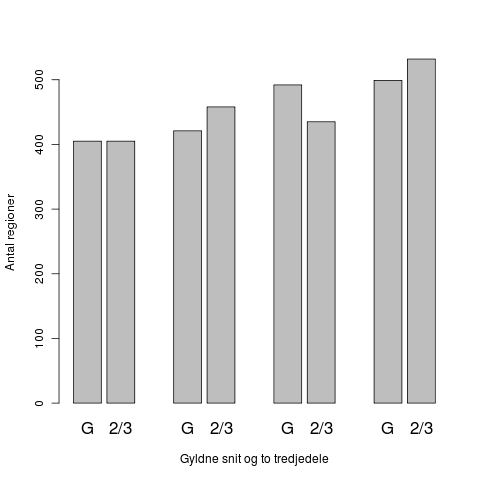
\includegraphics[width=0.6\textwidth]{afsnit/resultater/billeder/G_vs_to_tredjedeleU.png}
	\end{center}
	\caption{Procent vis antal regioner i de fire gyldne snit og deres tilhørene $\frac{2}{3}$ snit}
	\label{G_vs_to_trejedele_udvidet}
\end{figure}

\begin{table}[!h]
    \centering
    \begin{tabular}{|l|c|c|}
        \hline
            & Afvist & Ikke afvist  \\\hline
        1   &            & \checkmark   \\\hline
        2   &            & \checkmark   \\\hline
        3   & \checkmark$^{\textrm{*}}$ &              \\\hline
        4   & \checkmark &              \\\hline
        5   & \checkmark &    	\\\hline
        6   & \checkmark &              \\\hline
        7   &            &              \\\hline
        8   &            &              \\\hline
        9   &            & 	\\\hline
    \end{tabular}
    \caption[]{Hypoteser i forhold til den udvidet kørsel.
    $^{\textrm{*}}$Jvf. udregning \ref{tabel_real_dimensions}.
    }
    \label{hypoteser_udvidet}
\end{table}

} % Eh eh eh. Nallerne væk!

% vim: set tw=72 spell spelllang=da:


\section*{Opsummering}
Dette kapitel har præsenteret resultaterne fra to analyser på vores
datasæt fra WGA og holdt dem op imod en samling af hypoteser.
Resultaterne fra en kørslen med den naive vurdering af regioner, har dog
brugt en fejlbehæftet metode til udtrækning af regioner.  Den udvidede
vurdering af regioner retter selv op på denne fejl, men disse resultater
dækker ikke hele datasættet.

Konklusion-opsummering-ting. De vigtigste pointer.

Sidste kapitel vil kaste et blik tilbage på vores metoder og
implementering af disse, for at vurdere på hvilke områder der skal
sættes ind i senere fremtidigt arbejde.

}
% vim: set tw=72 spell spelllang=da:
